\subsection{Architektura systemu}
Projektowany system to „Portal do zarządzania zadaniami”, który służy jako poligon doświadczalny dla wdrażanych praktyk inżynierskich. System został zaprojektowany w~architekturze mikroserwisowej, co pozwala na pełną demonstrację procesów DevOps w~środowisku rozproszonym, w~tym niezależnego budowania, testowania i~wdrażania poszczególnych komponentów.
Przegląd całego systemu przedstawia rysunek~\ref{fig:system-overview}: ruch użytkownika trafia przez Traefik Ingress do aplikacji frontendowej oraz interfejsów REST usług \textit{users} i~\textit{tasks}, natomiast komunikacja między usługami odbywa się wyłącznie asynchronicznie --- przez tematy brokera Apache Pulsar. Usługa \textit{tasks} utrzymuje zasilany zdarzeniami lokalny model odczytu użytkowników (\texttt{KnownUser}), dzięki czemu walidacja nie wymaga synchronicznego wywołania usługi \textit{users}.

\begin{figure}[H]
    \centering
    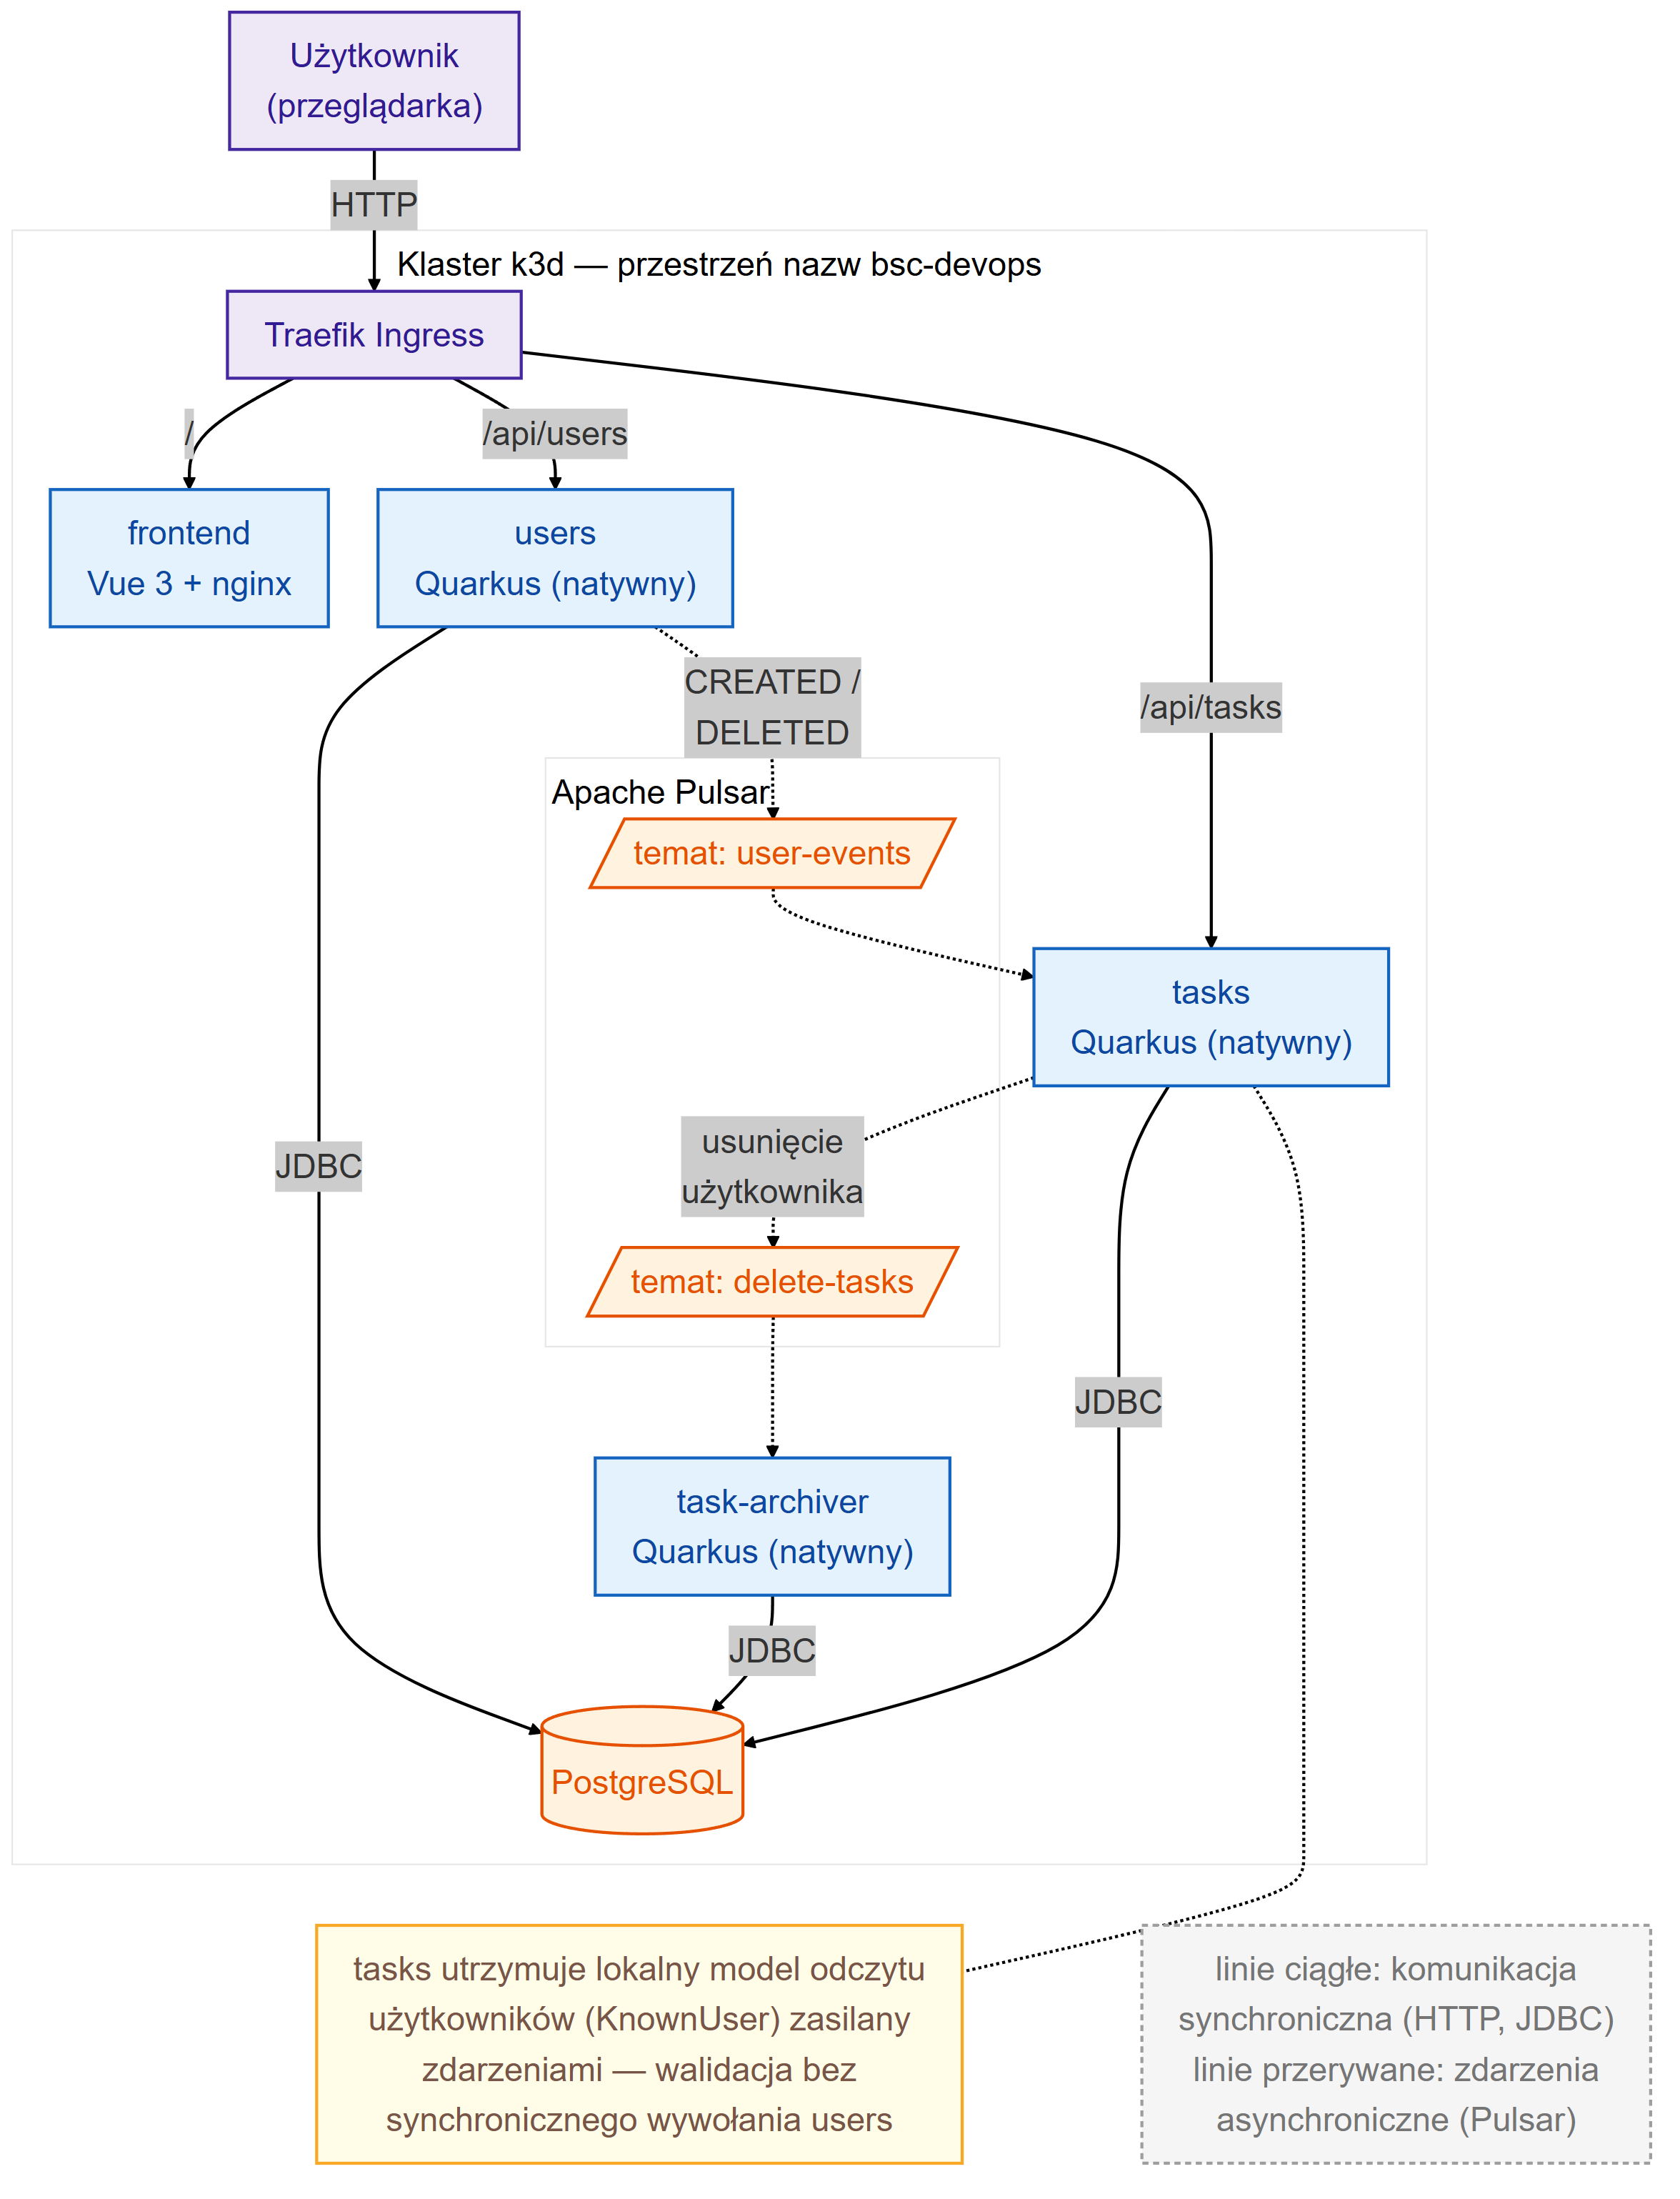
\includegraphics[width=0.9\textwidth]{img/diagrams/02-architektura/architektura-01-system-overview.png}
    \caption{Architektura systemu --- ścieżka synchroniczna (HTTP, JDBC) i~zdarzeniowa (tematy Apache Pulsar) w~jednym przeglądzie (opracowanie własne).}
    \label{fig:system-overview}
\end{figure}

W~warstwie technologicznej zdecydowano się na wykorzystanie ekosystemu Java z~frameworkiem \textit{Quarkus} (ADR-0003). 
Wybór ten podyktowany był charakterem środowiska uruchomieniowego, jakim jest Kubernetes. 
Quarkus, będący rozwiązaniem \textit{Kubernetes-native}, pozwala na znaczną optymalizację zużycia zasobów (pamięci RAM i~procesora) oraz skrócenie czasu uruchamiania aplikacji dzięki kompilacji z~wyprzedzeniem (ang. \textit{Ahead-of-Time}, AOT).
Jest to kluczowe w~architekturze mikroserwisowej, gdzie efektywność kosztowa i~szybkość skalowania są priorytetem.
Aplikacja została zaprojektowana zgodnie z~wytycznymi \textit{Twelve-Factor App}, co zapewnia jej pełną przenośność.

Głównym środowiskiem uruchomieniowym wykorzystywanym w~części praktycznej jest lokalny klaster Kubernetes (\textit{k3d}, ADR-0015).
Takie podejście pozwala na pełną odtwarzalność środowiska produkcyjnego na maszynie deweloperskiej, co jest zgodne z~ideą \textit{Cloud Native}.
Mimo skupienia na środowisku lokalnym, wszystkie zastosowane narzędzia i~konfiguracje (np. Helm, manifesty Kubernetes, aplikacje ArgoCD) są projektowane w~sposób \textit{cloud-agnostic}, umożliwiający ich przeniesienie do publicznych dostawców chmurowych (np. AWS).

\subsection{Struktura części praktycznej}
Opis części praktycznej został ustrukturyzowany w~sposób odzwierciedlający klasyczną pętlę cyklu życia oprogramowania (ang. \textit{DevOps Lifecycle}).
Każdy z~etapów pętli --- od planowania po monitorowanie --- został szczegółowo omówiony w~kontekście wybranych narzędzi i~metodyk.

Przyjęto formę opisu opartą na tzw. „kartach narzędzi”. Dla każdego z~kluczowych komponentów infrastruktury przedstawiono:
\begin{itemize}
    \item opis i~uzasadnienie wyboru danego rozwiązania (często poparte dokumentami ADR),
    \item fragmenty konfiguracji (\textit{Infrastructure as Code}, manifesty YAML, definicje procesów CI/CD),
    \item rolę narzędzia w~całym ekosystemie oraz dobre praktyki inżynierskie zastosowane przy jego konfiguracji.
\end{itemize}

Dzięki takiej strukturze można łatwo zrozumieć, jak poszczególne narzędzia współgrają ze sobą w~ramach kompleksowego procesu dostarczania oprogramowania, a~także jakie decyzje architektoniczne i~inżynierskie stoją za ich implementacją.

Poniższe sekcje szczegółowo opisują realizację kolejnych etapów pętli DevOps.
